\documentclass{article}
\usepackage{graphicx}
\usepackage[utf8]{inputenc}
\usepackage[table,xcdraw]{xcolor}
\usepackage[margin=1in]{geometry}
\usepackage{setspace}


\title{Tecnologias de Descoberta de Conhecimento\\
Lista de Exercícios I - Parte A}

\author{Pedro Augusto Duarte de Almeida}
\date{Setembro/2016}

\begin{document}

\maketitle

\section{Considere uma base de dados com informações sobre a frequência acadêmica de alunos. Nesse contexto, aponte o que poderiam ser um dado, uma informação e um conhecimento.}

\subsection{Dados}
\textbf{Dados} são códigos que constituem a matéria prima da informação, ou seja, é a informação não tratada. Os dados representam um ou mais significados que isoladamente não podem transmitir uma mensagem ou representar algum conhecimento.

\begin{table}[h]
\centering
\caption{Dados}
\label{dados}
\begin{tabular}{|l|l|l|l|l|}
\hline
N       & S & D          & idD & CH \\ \hline
Igor    & P & 2016-09-29 & 2   & 68 \\ \hline
Gabriel & A & 2016-09-29 & 4   & 34 \\ \hline
Pedro   & P & 2016-09-29 & 3   & 34 \\ \hline
\end{tabular}
\end{table}

\noindent
A tabela acima constitui apenas um conjunto de \textbf{Dados}, pois somente com ela não se pode estabelecer um contexto nem um significado. Podemos até imaginar alguns significados, mas não há como assegurar sua validade.
\noindent
\subsection{Informação:}
\textbf{Informações} são dados tratados. O resultado do processamento de dados são as informações. As informações têm significado, podem ser tomadas decisões ou fazer afirmações considerando as informações. 
\noindent
\textbf{Informação} é o sentido que um conjunto de dados tem para alguém. Um conjunto de Dados representa uma Informação, para uma pessoa, quando ela consegue perceber suas relações com outros Dados, que lhe definem um contexto e, ainda, com outros Dados e Informações que já lhe são familiares, estabelecendo  assim seu significado  para  ela. 
\singlespacing
\noindent
\textbf{Informação} é, portanto, a leitura que cada indivíduo faz de um conjunto de Dados, é o significado que lhe atribui ao internalizar esses Dados. 

\begin{table}[h]
\centering
\caption{Informação}
\label{info}
\begin{tabular}{|l|l|l|l|l|}
\hline
Nome    & Situação & Data       & idDisciplina & CargaHoraria \\ \hline
Igor    & P        & 2016-09-29 & 2            & 68           \\ \hline
Gabriel & A        & 2016-09-29 & 4            & 34           \\ \hline
Pedro   & P        & 2016-09-29 & 3            & 34           \\ \hline
\end{tabular}
\end{table}
\noindent
Na tabela acima, se for esclarecido que se trata de um registro de frequência de alunos que especifica o nome do aluno, a data da chamada, a situação do aluno naquela data (P de Presente ou A de Ausente), e id da disciplina; e se esses termos e conceitos fazem sentido, o usuário passa a entender o contexto e o significado dos Dados, que passam a constituir uma Informação. Para um usuário não habituado ao funcionamento de frequência de alunos numa universidade, os Dados podem fazer menos sentido, não transmitindo a mesma Informação.

\subsection{Conhecimento:}

É a capacidade, adquirida por alguém, de interpretar e operar sobre um conjunto de Informações. Essa capacidade é criada a partir das relações que ele estabelece  sobre o conjunto de Informações, e desse conjunto com outros conjuntos que já lhe são  familiares, que lhe permitem compreende-lo e tirar conclusões sobre ele e a partir dele.
\singlespacing
\noindent
Com referência à mesma tabela acima, se o usuário tem conhecimento sobre o funcionamento da frequência academia dos alunos, o mesmo é capaz de interpretar as informações com  maior profundidade, por exemplo, deduzindo o número de faltas que um aluno pode ter para ser reprovado numa determinada disciplina, baseando-se na carga horária total da mesma juntamente com alguma regra de negócio que estipula a porcentagem máxima de faltas permitida pela instituição de ensino. 
\begin{table}[h]
\centering
\caption{Dados x Informação x Conhecimento}
\label{my-label}
\begin{tabular}{|l|l|l|}
\hline
Dado          & Informação              & Conhecimento                          
\\ \hline
Nome do Aluno & \begin{tabular}[c]{@{}l@{}}Presente ou Ausente;\\ Data da Presença ou Ausência;\\ Disciplina\end{tabular} & \begin{tabular}[c]{@{}l@{}}Estudo do perfil do ano;\\ Previsão de frequência até o final do semestre;\\ Cálculo de faltas restantes permitidas\end{tabular} \\ \hline
\end{tabular}
\end{table}

\section{Considerando a plataforma Data Viva, faça:}
\subsection{Dê uma visão geral sobre os dados que podem ser encontrados nessa plataforma}
Dados sobre as exportações, atividades econômicas locais, ocupações e educação em todo o Brasil.
\subsection{Identifique pelo menos dois tipos de técnicas de data mining que poderiam ser aplica das nas bases de dados da plataforma}
\begin{enumerate}
    \item Descoberta de Associações: Associar a compra de um produto x com um produto y
    \item Regressão: Predição da soma da biomassa presente em uma floresta; a predição do risco de determinados investimentos;
\end{enumerate}
\subsection{Aponte um potencial tipo de conhecimento que um poderia ser extraído dessa base de dados}
\begin{itemize}
    \item Números das profissões com as melhores médias salariais de cada estado;
    \item Melhores opções de investimento em cada estado;
    \item Tomar decisão sobre onde instalar uma startup e como integrá-la à cadeia de suprimentos das empresas locais;
    \item Nome e localização das universidades que mais possuem formandos por semestre.
\end{itemize}

\section{Pesquisa no site Kaggle uma competição que chame sua atenção e descreva:}
\subsection{Objetivo da competição}
Nesta competição, é disponibilizado participantes uma tabela com dados (como nome, idade, valor da passagem, etc) de 891 passageiros (dataset de treino) que estavam a bordo do Titanic e seu respectivo destino após o acidente (faleceu/sobreviveu). O objetivo é criar modelos que corretamente prevejam o destino dos 418 passageiros restantes (dataset de teste).
\subsection{Os dados disponibilizados}
Para cada passageiro:
\begin{enumerate}
    \item Nome;
    \item Classe;
    \item Sexo;
    \item Idade;
    \item Número de irmãos(as)/esposos(as) à bordo;
    \item Número de pais;
    \item Número do ticket;
    \item Tarifa;
    \item Localização da cabine;
    \item Porto de embarque
    \item Indicador de destino final (0 = Não sobreviveu 1 = Sobreviveu)
\end{enumerate}

\subsection{Como você pensaria em resolver o problema apresentado na competição}
\begin{enumerate}
    \item Importar todos os dados fornecidos pela competição
    \item Excluir informações que serão irrelevantes para minha análise, como o número do ticket, tarifa, e o porto de embarque
    \item "Mulheres e crianças primeiro". Verificar a proporção de sobreviventes entre homens e mulheres. Filtrar os dados pelo sexo e a idade de cada passageiro
    \item Em posse do conhecimento da proporção de sobreviventes entre homens e mulheres, cruzar com os dados dos passageiros com destino (sobreviveu ou não) desconhecido.
\end{enumerate}


\section{Faça uma análise comparativa entre as metodologias KDD e SEMMA. Nessa análise você deverá:}
\subsection{Descrever cada uma das metodologias e suas etapas}
\subsubsection{KDD}
O processo KDD é o processo de usar métodos de Data Mining para extrair o que é considerado conhecimento em acordo com a especificação de metricas e limiares. São considerados 5 estágios:
\begin{enumerate}
    \item Seleção: Esse estágio consiste em criar uma coleção de dados alvo, ou focar em um sub conjunto de variáveis ou dados simples, nos quais a descoberta e feita.
    \item Pré Processamento: Esse estágio consiste na limpeza dos dados alvo e o seu pre processamento visando obter dados consistentes.
    \item Transformação: Esse estágio consiste na transofrmação dos dados reduzindo as suas dimensões ou métodos de transformação.
    \item Data Mining: Esse estágio consiste na busca por padrões de interesse numa particular forma representacional, dependendo do objetivo do data mining.
    \item Interpretação/Avaliação: Esse estágio consiste na interpretação e avaliação dos padrões mineirados.
\end{enumerate}
\noindent
O processo KDD é interativo e iterativo, envolvendo vários passos com várias decisões sendo feitas pelo usuário. Adicionalmente, o processo KDD deve proceder pelo desenvolvimento do conhecimento do dominio da aplicação, o conhecimento relevante pŕevio e os objetivos do usuário final.

\subsubsection{SEMMA}
A metodologia SEMMA, foi desenvolvida pela SAS, que define Data Mining como o processo de extrair informação valiosa e relações complexas de um grande volume de dados, dividiram o processo de Data Mining em cinco fases que compõe o acrónimo SEMMA:
\begin{enumerate}
    \item Amostragem: Recolha de uma amostra significativamente grande para ser representativa da população e pequena o suficiente para ser manipulada rapidamente.
    \item Explorar: Exploração estatística e gráfica dos dados para se ter ideia à partida de algum padrão, tendências ou anomalias nos dados.
    \item Modificar: Modificação dos dados criando, seleccionando e transformando variáveis para obter nova informação. Identificação de pontos extremos, tratamento de valores omissos e segmentação da base de dados.
    \item Modelo: Ajustamento de modelos predicativos, modelação das variáveis objectivo usando algoritmos baseados em árvores de decisão, regressões, redes neuronais ou modelos definidos pelos analistas.
    \item Avaliar: Esse estágio consiste na avaliação dos dados, avaliando a usabilidade e confiabilidade dos resultados do processod e Data Mining e a estimativa de quão bem é executado.
\end{enumerate}
\noindent
Embora o processo SEMMA seja independente da ferramente de Data Mining escolhida, o SEMMA e relacionado ao software SAS Enterprise Minere pretende guiar o usuário na implementação de aplicações de Data Mining. SEMMA oferece uma forma fácil de entender processo, permitindo o desenvolvimento e a manutenção de forma organizada e adequada em projetos de Data Mining.
\subsection{Apresentar as principais vantagens de uma em relação a outra}
Comparando os estágios do KDD com os do SEMMA, em primeira instância, afirmamos que são equivalentes:
\begin{itemize}
    \item Sample (Amostra) pode ser identificada com Selection (Seleção)
    Explore (Explorar) pode ser identificado com Pre Processing (Pré Processamento)
    \item Modify (Modificar) pode ser identificado com Transformation (Transformação)
    \item Model (Modelo) pode ser identificado com Data Mining (Mineração de Dados)
    \item Assess (Avaliação) pode ser identificado com Interpretation/Evaluation (Interpretação/Avaliação)
\end{itemize}
\noindent
Examinando como um todo, podemos afirmar que os cinco estágios do processo SEMMA podem ser vistos como uma implementação pratica dos cinco estágios do processo KDD, desde que o SEMMA é diretamente ligado ao software SAS Enterprise Miner.

\section{Resolva pelo menos 3 questões entre os exercícios propostos (1 a 5) no final capítulo 8 do livro}
\subsection{Questão 1:}
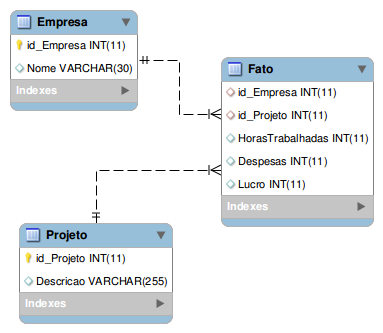
\includegraphics[scale=0.7]{1.png}
\subsection{Questão 2:}
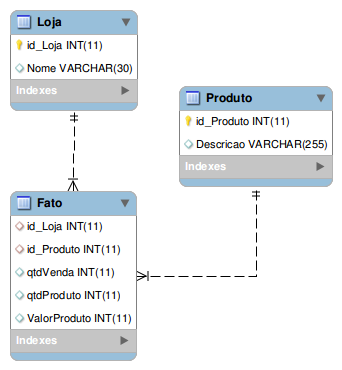
\includegraphics[scale=0.7]{2.png}
\subsection{Questão 4:}
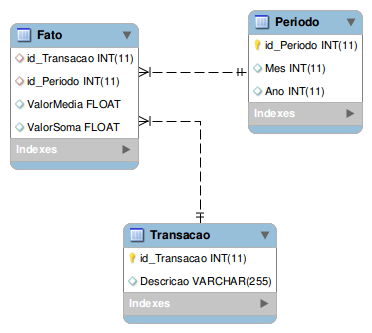
\includegraphics[scale=0.7]{4.png}

\end{document}